I noen systemer er det viktig at ikke strømmen
eller spenningen skifter retning.
Hvis man har utgangspunkt i vekselstrøm kan man forskyve den
ved å legge til en likestrømsspenning minst like sterk
som $V_{P}$.
\\
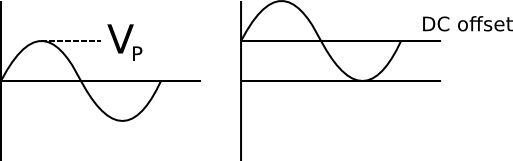
\includegraphics[width=0.5\textwidth]{./img/dcoffset}
